\documentclass{article}
\usepackage{tikz}
\usetikzlibrary{arrows.meta,positioning,calc,shapes.geometric}
\pagestyle{empty}
\begin{document}
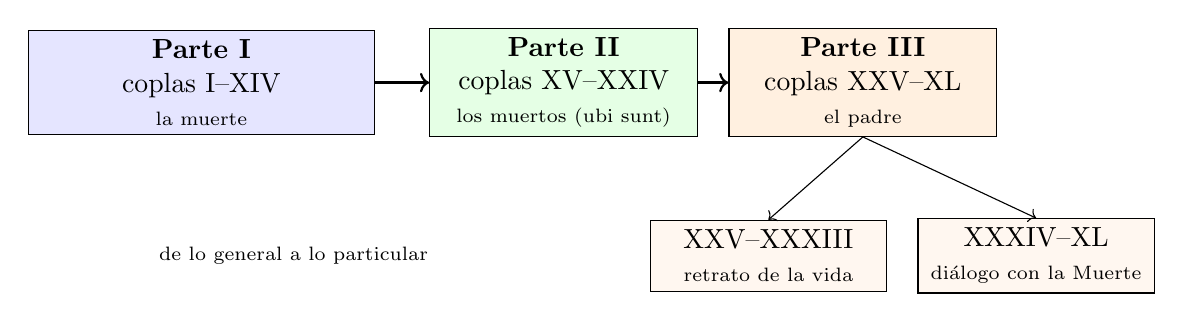
\begin{tikzpicture}
\tikzset{every node/.append style={align=center}}

\node[draw, fill=blue!10, minimum width=4.4cm, minimum height=1.2cm, align=center] (a) at (0,0) {\textbf{Parte I}\\ coplas I--XIV\\ \scriptsize la muerte};
\node[draw, fill=green!10, minimum width=3.4cm, minimum height=1.2cm, align=center] (b) at (4.6,0) {\textbf{Parte II}\\ coplas XV--XXIV\\ \scriptsize los muertos (ubi sunt)};
\node[draw, fill=orange!12, minimum width=3.4cm, minimum height=1.2cm, align=center] (c) at (8.4,0) {\textbf{Parte III}\\ coplas XXV--XL\\ \scriptsize el padre};
\draw[->, thick] (a) -- (b); \draw[->, thick] (b) -- (c);
\node[draw, fill=orange!6, minimum width=3.0cm, minimum height=0.9cm, align=center] (c1) at (7.2,-2.2) {XXV--XXXIII\\ \scriptsize retrato de la vida};
\node[draw, fill=orange!6, minimum width=3.0cm, minimum height=0.9cm, align=center] (c2) at (10.6,-2.2) {XXXIV--XL\\ \scriptsize diálogo con la Muerte};
\draw[->] (c.south) -- (c1.north); \draw[->] (c.south) -- (c2.north);
\node[font=\scriptsize, anchor=east] at (3.0,-2.2) {de lo general a lo particular};

\end{tikzpicture}
\end{document}
